\chapter{รายละเอียดการปฏิบัติงาน}
\label{chapter:related-theory}

เริ่มสหกิจศึกษาโดยปฏิบัติงานที่ บริษัท วงใน มีเดีย จำกัด (สำนักงานใหญ่) ตั้งแต่วันที่ 4 มิถุนายน พ.ศ.2562 จนถึง 29 พฤศจิกายน พ.ศ.2562 รวมเป็นระยะเวลาประมาณ 6 เดือน โดยในการปฏิบัติงานต่าง ๆ ในช่วงสหกิจศึกษา มีรายละเอียดดังต่อไป

\section{ตำแหน่ง/หน้าที่ของงานที่ได้รับมอบหมาย}
ปฏิบัติงานด้วยตำแหน่ง Software Engineer (Back-end) ทำหน้าที่รับผิดชอบในการสร้างและดูแลระบบ Backend ของเว็บไซต์ wongnai.com เพื่อให้ผู้ใช้งานในทุกแพลตฟอร์ม เช่น Web และ Mobile Application สามารถทำงานร่วมกันได้อย่างมีประสิทธิภาพ, ควบคุมคุณภาพของโค้ดให้มีคุณภาพที่ดี ทำงานได้ถูกต้อง ทดสอบและดูแลได้ง่าย มีความยืดหยุ่นพร้อมรับการเปลี่ยนแปลงในอนาคต

\section{รายละเอียดของโครงงานที่รับผิดชอบ}
โครงงานที่รับผิดชอบคือ ระบบจัดการโฆษณาแบบจำกัดจำนวนการคลิกและการแสดงโฆษณา แต่เดิมนั้นลูกค้าจะสามารถลงโฆษณาร้านของตนเองกับทาง Wongnai ได้แค่ตามช่วงเวลาที่ตกลงกันไว้ ยกตัวอย่างเช่น ลูกค้ามาขอติดต่อลงโฆษณาเป็นระยะเวลา 30 วัน ตั้งแต่วันที่ 1 กันยนยน จนถึง 30 กันยายน เป็นต้น ระบบที่พัฒนาขึ้นใหม่นั้นจะทำให้ลูกค้าสามารถลงโฆษณากับทาง Wongnai อีกรูปแบบหนึ่งโดยการลงโฆษณาแบบจำกัดจำนวนการแสดงโฆษณาและการคลิก เช่น หากลงโฆษณาไว้แล้วแสดงโฆษณาเกิน 10,000 ครั้ง หรือมีผู้ที่คลิกเข้าไปในโฆษณาครบ 5,000 คน ระบบก็จะหยุดแสดงโฆษณานั้นโดยอัตโนมัติ และยังมีระบบที่สามารถรายงานโฆษณาที่ลูกค้าลงไว้ได้อย่างอัตโนมัติอีกด้วย

\section{รายละเอียดของงานที่ปฏิบัติ}
ในการปฏิบัติงาน ได้มีการนำเทคโนโลยีและเครื่องมือต่าง ๆ มาใช้งาน เพื่อให้การพัฒนาระบบเป็นไปอย่างราบรื่น, รวดเร็ว และสามารถทำงานร่วมสมาชิกทีมคนอื่น ๆ ได้อย่างมีประสิทธิภาพ  โดยเทคโนโลยีและเครื่องมือต่าง ๆ นั้น ได้แก่
\begin{enumerate}
	\item IntelliJ IDEA
	
	IntelliJ IDEA เป็น Integrate Development Environment (IDE) สำหรับใช้ในการพัฒนาซอฟต์แวร์ที่ใช้ Java Virtual Machine (JVM) โดยเฉพาะ มีระบบ Suggestion และ Auto Completion ที่ทำให้การทำงานเป็นไปอย่างราบรื่นและรวดเร็ว
	
	\item Sequel Pro
	
	Sequel Pro เป็นแอปพลิเคชันสำหรับจัดการฐานข้อมูล MySQL
	
	\item Postman
	
	Postman เป็นแอปพลิเคชันสำหรับสร้าง API Request เช่น REST, SOAP, GraphQL เพื่อทดสอบการทำงาน API ของ Server และสามารถตรวจสอบ Response ที่ส่งกลับมาได้
	
	\item Visual Studio Code
	
	Visual Studio Code เป็น Text Editor ที่รองรับได้หลากหลายภาษา มีระบบ Syntax Highlighting ในการตรวจสอบ Syntax ของโค้ด และสามารถติดตั้งส่วนขยายต่าง ๆ เพิ่มเติมได้ตามความเหมาะสมในการทำงาน
	
	\item GitKraken
	
	GitKraken เป็น Git GUI Client ที่ทำให้สามารถใช้งาน Git ได้อย่างสะดวกสบาย
	
	\item Asana
	
	Asana คือระบบออนไลน์ที่คอยแสดง Workflow ของสมาชิกทีม ทำให้สมาชิกคนอื่น ๆ ในทีมสามารถทราบสถานะงานของแต่ละคนได้อย่างรวดเร็ว
	
	\item Java
	
	Java เป็นภาษาคอมพิวเตอร์ประเภท Object-Oriented ที่สามารถนำ bytecode ที่ได้จากการ Compile ไปใช้งานบนคอมพิวเตอร์เครื่องไหนก็ได้ที่มี Java Virtual Machine (JVM)
	
	\item Python
	
	Python เป็นภาษาคอมพิวเตอร์ระดับสูงที่ใช้ Python Interpreter มีจุดเด่นที่สามารถอ่านและทำความเข้าใจโค้ดได้ง่าย โดย Python Interpreter นั้น สามารถติดตั้งได้ในหลากหลายระบบปฏิบัติการ 
	
	\item MySQL
	
	MySQL เป็นตัวจัดการฐานข้อมูลแบบ Relational (Relational Database Management: RDBMS) ที่เป็น Open source
	
	\item Google BigQuery
	
	Google BigQuery เป็น Data Warehouse บน Cloud ที่ให้บริการโดย Google และสามารถใช้ SQL เพื่อใช้งาน Google BigQuery ได้
	
	\item Git
	
	Git คือ Version Control ที่สามารถติดตามและควบคุมการเปลี่ยนแปลงของโค้ดได้ เพื่อให้ Software Engineer คนอื่น ๆ สามารถทำงานร่วมกันได้อย่างมีประสิทธิภาพ
	
	\item Docker
	
	\item Kubernetes

	Kubernetes คือ เทคโนโลยีสำหรับจัดการ Cluster (กลุ่มเครื่อง Server) สามารถจัดการ Container ที่กำลังรันระบบเพื่อให้สามารถทำงานได้อย่างต่อเนื่อง มี downtime เป็นศูนย์ ~\cite{kubernetes}
	
\end{enumerate}

ระบบจัดการโฆษณาแบบจำกัดจำนวนการคลิกและการแสดงโฆษณาที่พัฒนาขึ้นมานั้น ประกอบด้วยเซอร์วิสต่าง ๆ ได้แก่

\begin{enumerate}
	\item Wongnai Core
	
	Wongnai Core เป็นระบบ Back-end หลักของ Wongnai ถูกพัฒนาด้วยภาษา Java ทำหน้าที่ให้บริการหลาย ๆ อย่าง โดยหน้าที่ของ Wongnai Core ที่เกี่ยวข้องกับระบบจัดการโฆษณาแบบจำกัดจำนวนการคลิกและการแสดงโฆษณา คือการควบคุมการแสดงผลโฆษณาของเว็บไซต์ wongnai.com และแอปพลิเคชัน Wongnai และคอยประมวลผลเมื่อได้รับข้อมูลจำนวนผู้ชมและผู้ที่คลิกเข้าไปในโฆษณาล่าสุดจาก Analytics Data Updater เพื่อนำไปพิจารณาต่อว่าควรจะนำโฆษณาที่แสดงอยู่ออกหรือไม่ โดยดูจากจำนวนผู้ชมและผู้ที่คลิกเข้าไปดูโฆษณาทั้งหมดว่าเกินกว่าตัวเลขที่จำกัดไว้ตามที่ตกลงกันไว้หรือไม่ ถ้าเกินแล้วก็จะหยุดการแสดงผลของโฆษณานั้น ๆ
	
	\item Analytics Data Pipeline
	
	Analytics Data Pipeline เป็นระบบขนาดเล็กที่ถูกพัฒนาด้วยภาษา Python ทำหน้าที่รวบรวมข้อมูลส่วนที่เราต้องการจากตารางข้อมูลขนาดใหญ่ตารางเดียวใน Google BigQuery โดยตารางข้อมูลขนาดใหญ่ดังกล่าวนั้น จะจัดเก็บข้อมูลที่ฝั่งไคลเอนต์ส่งมาบันทึกไว้ ซึ่งจะส่งข้อมูลเกี่ยวกับการกระทำต่าง ๆ ที่เกิดขึ้นบนฝั่งไคลเอนต์ เช่น ตำแหน่งที่รูปภาพในระบบถูกนำไปแสดงบนไคลเอนต์แพลตฟอร์ม, ตำแหน่งต่าง ๆ บนเว็บไซต์ที่มีผู้ใช้คลิกลงไป เป็นต้น หน้าที่ที่เกี่ยวข้องกับระบบจัดการโฆษณาแบบจำกัดจำนวนการคลิกและการแสดงโฆษณาสำหรับ Analytics Data Pipeline คือการรวบรวมข้อมูลส่วนที่เป็นข้อมูลการแสดงโฆษณาและข้อมูลผู้ใช้งานที่คลิกเข้าไปที่โฆษณา ไปจัดเก็บแยกไว้ในอีกตารางหนึ่งใน Google BigQuery เพื่อให้สะดวกต่อการนำข้อมูลไปใช้งานต่อ
	
	\item Analytics Data Updater
	
	Analytics Data Updater เป็นระบบขนาดเล็กที่พัฒนาด้วยภาษา Python ทำหน้าที่นำข้อมูลการแสดงโฆษณาและข้อมูลผู้ใช้งานที่คลิกเข้าไปที่โฆษณาที่ Analytics Data Pipeline รวบรวมเป็นตารางขนาดเล็กไว้ให้แล้ว ส่งไปอัปเดตที่ Wongnai Core เพื่อให้ Wongnai Core ทำการประมวลผลเพื่อพิจารณาดูว่าควรจะเอาโฆษณาออกแล้วหรือไม่
	
	\item Advertisement Report Service
	
	เป็นระบบที่ถูกพัฒนาด้วยภาษา Java ทำหน้าที่สร้างรายงานของโฆษณาที่มีข้อมูลเกี่ยวกับสถิติต่าง ๆ ของโฆษณา ได้แก่ จำนวนผู้ชมโฆษณาต่อวัน, จำนวนผู้ที่คลิกเข้าไปในโฆษณาต่อวัน, จำนวนการคลิกและการชมที่ยังคงเหลืออยู่จากที่ตกลงกันไว้
\end{enumerate}

กระบวนการทำงานของระบบจัดการโฆษณาแบบจำกัดจำนวนการคลิกและการแสดงโฆษณา จะเป็นไปตามแผนผังดังต่อไปนี้

\section{ลักษณะขั้นตอนการทำงาน}
ทีม Development ของบริษัท วงใน มีเดีย จำกัด (สำนักงานใหญ่) จะถูกแบ่งออกเป็นทีมย่อย ๆ ตามประเภทของฟังก์ชันที่รับผิดชอบ เรียกว่า Squad ซึ่งจะเป็นทีมแบบ Cross-Functional กล่าวคือ ภายในทีมจะประกอบไปด้วยหลาย ๆ ฝ่าย ได้แก่ Project Manager, Software Engineer (Front-end), Software Engineer (Back-end), Software Engineer (iOS), Software Engineer (Android) และ Quality Assurance Engineer

แต่ละ Squad นั้นจะทำงานโดยใช้ Scrum เป็นหลัก Scrum จะทำงานเป็นวงรอบ (Sprint) แต่ละรอบนั้นจะเท่ากับ 1 สัปดาห์ แต่ภายหลังได้มีการปรับเปลี่ยนไปเป็นรอบละ 2 สัปดาห์ โดยจะกิจกรรมที่สำคัญต่าง ๆ ดังต่อไปนี้
\begin{enumerate}
	\item Sprint Planning
	
	เป็นการประชุมตอนต้นรอบ เพื่อรับมอบหมายงานจาก Project Manager และเป็นการประชุมเพื่อปรึกษาหาวิธีการทำงานและวิธีการแก้ไขปัญหาต่าง ๆ ที่เกี่ยวกับงานที่ได้รับมอบหมาย
	
	\item Daily Meeting
	
	เป็นการประชุมแบบสั้น ๆ ประจำวัน มีจุดประสงค์เพื่อให้สมาชิกทีมรับทราบความคืบหน้าของงานที่แต่ละคนกำลังทำอยู่และทราบปัญหาที่เกิดขึ้นระหว่างการทำงาน
	
	\item Backlog Refinement Meeting
	
	เป็นการประชุมตอนกลางรอบ เพื่อพิจารณาว่างานที่ได้รับมอบหมายมา มีขนาดใหญ่หรือเล็กกว่าที่วางแผนไว้หรือไม่ และปรึกษาหาทางแก้ไขที่เหมาะสมกับสถานการณ์
	
	\item Retrospective Meeting
	
	เป็นการประชุมตอนปลายรอบ เพื่อสรุปการทำงานที่ได้ทำไปในรอบ และให้สมาชิกภายในทีมอธิบายปัญหาที่เกิดขึ้นในรอบ รวมไปถึงเรื่องราวดี ๆ ที่เกิดขึ้นในรอบด้วย เพื่อนำไปปรับปรุงการทำงานในรอบถัดไป
\end{enumerate}

การติดต่อสื่อสารภายในองค์กรจะใช้ Slack เป็นหลัก สถานะของงานภายในทีมสามารถดูได้จาก Kanban Board ซึ่งเป็นบอร์ดที่ตั้งอยู่ในพื้นที่ทำงาน และ Asana ซึ่งเป็นระบบออนไลน์ที่จะทำให้สมาชิกภายในทีมสามารถทราบสถานะของงานได้อย่างรวดเร็ว ภายในกระบวนการทำงาน สถานะของงานจะเป็นไปตามดังต่อไปนี้

\begin{enumerate}
	\item To do
	
	งานที่ยังไม่ได้เริ่มทำ แต่อยู่ในรอบแล้วจะมีสถานะเป็น To do
	
	\item In progress
	
	งานที่กำลังทำอยู่จะมีสถานะเป็น In progress
	
	\item Review
	
	เมื่องานที่ทำอยู่เสร็จแล้ว ก่อนที่จะนำงานส่วนที่ทำเข้าไปในระบบ Beta ซึ่งเป็นระบบที่มีไว้ทดสอบก่อนที่จะใช้งานจริง โค้ดที่เขียนขึ้นมาจะต้องผ่านการตรวจสอบจาก Software Engineer คนอื่นอย่างน้อย 2 คนก่อน จึงจะสามารถส่งไปให้ Quality Assurance Engineer ทำการทดสอบต่อได้
	
	\item Review passed
	
	เมื่องานที่ทำอยู่ผ่านการตรวจสอบโดย Software Engineer คนอื่นครบ 2 คนแล้ว งานจะอยู่ในสถานะ Review passed 
	
	\item Testing
	งานที่อยู่ในสถานะ Review passed จะถูกส่งต่อให้ Quality Assurance Engineer ทดสอบ ซึ่งก่อนที่จะให้ Quality Assurance Engineer ทดสอบนั้น จะต้องเตรียมวิธีการทดสอบและเตรียมข้อมูลให้เรียบร้อยก่อน
	
	\item Test passed
	
	เมื่อ Quality Assurance Engineer ทดสอบเสร็จแล้ว งานจะอยู่ในสถานะ Test passed สามารถนำงานเข้าระบบ Beta ได้เลย
	
	\item Done
	
	เมื่อนำงานขึ้นระบบ Beta เสร็จแล้ว งานจะมีสถานะเป็น Done แต่อย่างไรก็ตาม เจ้าของงานจะต้องติดตามงานของตัวเองจนกว่างานจะขึ้นอยู่บนระบบที่ใช้งานจริง
\end{enumerate}

โดยส่วนมากแล้ว ถ้าเป็นงานที่เป็นการเขียนโค้ด จะมีกระบวนตามที่กล่าวมา แต่อย่างไรก็ตามงานบางชนิดไม่จำเป็นต้องทำตามกระบวนการอย่างเคร่งครัดก็ได้ ขึ้นอยู่กับความเหมาะสมของงานว่าควรจะเป็นแบบไหน เช่น งานบางชิ้นที่เป็นการสร้างเครื่องมือให้กับพนักงานฝ่ายอื่นในบริษัทใช้ เราสามารถให้พนักงานฝ่ายนั้น ซึ่งเป็นผู้ใช้งานโดยตรงเป็นผู้ทดสอบงานของเราแทนก็ได้ เพื่อที่จะนำความคิดเห็นไปปรับปรุงงานได้อย่างตรงจุดที่สุด

การทำงานของทีม Development ที่เป็นการเขียนโค้ดจะใช้ Test Driven Development (TDD) เป็นหลัก เป็นการเขียนชุดทดสอบของโค้ดขึ้นมาก่อน แล้วรันชุดสอบให้เกิดข้อผิดพลาด จากนั้นจึงเขียนโค้ดเพื่อแก้ไขไม่ให้เกิดข้อผิดพลาดนั้น ระหว่างการเขียนโค้ดจะต้องคอยคำนึงถึงคุณภาพของโค้ด หากมีโค้ดส่วนที่ทำงานซ้ำกันจะต้องทำการ Refactoring โค้ดส่วนนั้นด้วย

\begin{figure}[!h]
	\centering
	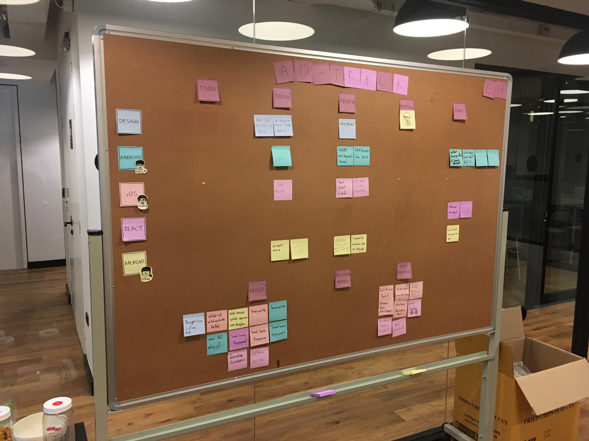
\includegraphics[width=0.8\textwidth]{kanban-board.png}  
	\caption{Kanban Board ที่ตั้งอยู่ในพื้นที่ทำงาน}
	\label{Fig:kanban-board}
\end{figure}

\begin{figure}[!h]
	\centering
	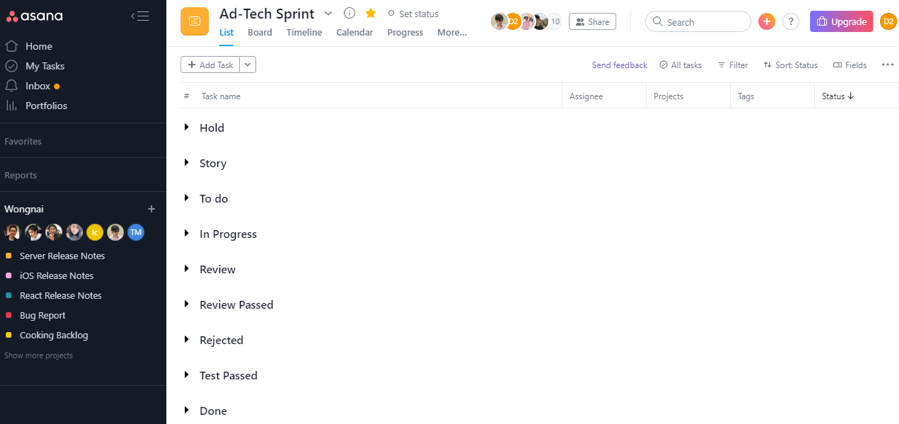
\includegraphics[width=1\textwidth]{asana.png}  
	\caption{ตัวอย่างของโปรแกรม Asana}
	\label{Fig:asana}
\end{figure}